\documentclass{article}
\usepackage[margin=1in]{geometry}
\usepackage{problemset}
\showsolntrue

% Custom commands
\newcommand{\R}{\mathbb{R}}
\newcommand{\X}{\mathcal{X}}
\newcommand{\Y}{\mathcal{Y}}
\newcommand{\E}{\mathbb{E}}
\newcommand{\V}{\text{Var}}
\renewcommand{\P}{\mathbb{P}}
\newcommand{\x}{\mathbf{x}}
\newcommand{\w}{\mathbf{w}}

\begin{document}

\pstitle{%
    COGS 181A%
}{
    Homework 2%
}[due Tuesday, January 27 at 11:59PM]

\textbf{Instructions:} Answer the questions below, attach your code, and insert figures to create a PDF file; submit your file via Gradescope. You may look up the information on the Internet, but you must write the final homework solutions by yourself.

\textbf{Late Policy:} 5\% of the total points will be deducted on the first day past due. Every 10\% of the total points will be deducted for every extra day past due.

\textbf{System Setup:} You can install Anaconda to setup the Jupyter Notebook environment. Most packages have been already installed in Anaconda. If some package is not installed, you can use \texttt{pip} to install the missing package, that is, just type \texttt{pip install PACKAGE\_NAME} in the terminal.

\begin{probset}
% --- Problem 1 ---
\begin{prob}[\textbf{(10 points) Conceptual Questions}]
    \begin{subprobset}
    \begin{subprob}
    Is the following statement true or false? For inputs of two-dimensional features $\x = (x_1, x_2)$, a perceptron classifier cannot solve the XOR problem (Figure 1), but a logistic regression classifier can.

    \begin{figure}[H]
        \centering
            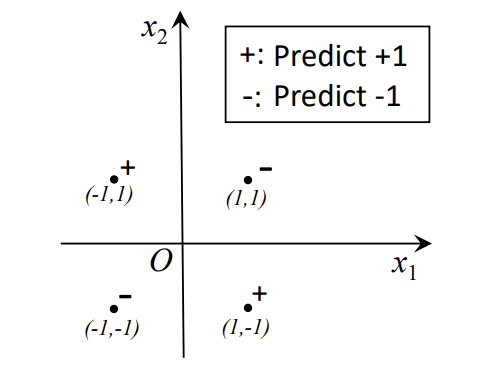
\includegraphics[width=0.3\textwidth]{Images/figure_1.png}
        \caption{The XOR Problem}
    \end{figure}

    \begin{soln}
            False, a logistic regression classifier cannot solve the XOR problem since it's not linearly separable.
        \end{soln}
    \end{subprob}

    \begin{subprob}
        Choose \textbf{all} the valid linear classifiers from the options below:

        \begin{enumerate}[label=\Alph*.]
            \item Perceptron.
            \item Logistic regression classifier.
            \item Multi-layer neural networks classifier.
        \end{enumerate}

        \begin{soln}
            A and B
        \end{soln}
    \end{subprob}

    \begin{subprob}
        Choose \textbf{all} the valid descriptions about \textbf{gradient descent} from the options below:

        \begin{enumerate}[label=\Alph*.]
            \item The global minimum can always be reached by using gradient descent.
            \item Every gradient descent iteration can always decrease the value of the loss function even when the gradient of the objective function is zero.
            \item When the learning rate is very large, some iterations of gradient descent may not decrease the value of the loss function.
            \item With different initial weights, the gradient descent algorithm may lead to different local minima.
            \item None of the above is valid.
        \end{enumerate}

        \begin{soln}
            C and D
        \end{soln}
    \end{subprob}

    \begin{subprob}
        Choose \textbf{all} the valid descriptions about the \textbf{stochastic gradient descent} algorithm
        from the options below:
        \begin{enumerate}[label=\Alph*.]
            \item Stochastic gradient descent (SGD) always finds the global optimal solution.
            \item Stochastic gradient descent (SGD) is typically more computationally efficient than standard gradient descent (GD).
            \item Stochastic gradient descent (SGD) is typically more memory-demanding than standard gradient descent (GD).
            \item Stochastic gradient descent (SGD) can be used to avoid bad local optima.
            \item Stochastic gradient descent (SGD) uses a fixed learning rate.
        \end{enumerate}

        \begin{soln}
            B and D
        \end{soln}
    \end{subprob}

    \begin{subprob}
        In this question, we will apply the perceptron learning algorithm to solve a binary classification problem: We need to predict a binary label $y \in \{-1, +1\}$ for a feature vector $\x = [x_0, x_1]^\top$. The decision rule of the perceptron model is defined as:

        \begin{align} 
            f(\x; \w, b) = \begin{cases}
                +1, & \text{if } \w \cdot \x + b \geq 0 \\
                -1, & \text{otherwise}
            \end{cases}
        \end{align}

        where $\w = [w_0, w_1]^\top$ is the weight vector, and $b$ is the bias scalar. Given a training dataset $S_\text{training} = \{(\x_i, y_i), i = 1, \ldots, n\}$, the outline of the perceptron algorithm is shown below:

        \begin{itemize}
            \item Initialize weight $\w$ and bias $b$.
            \item If not all data points in $S_\text{training}$ are correctly predicted:
                \begin{itemize}
                    \item Obtain the prediction for each feature vector in $S_\text{training}$.
                    \item If the prediction is wrong, then update the parameters $\w$ and $b$.
                \end{itemize}
            \item Otherwise return current weight $\w$ and bias $b$.
        \end{itemize}

        In this problem, you will implement a perceptron algorithm. Suppose $X$ is the matrix of all feature vectors $\x_i$ and $Y$ is the matrix of all labels $y_i$ in the training set $S_\text{training}$.

        Besides, assume a function \texttt{calc\_error(X, Y, W, b)} is given, which computes the error from the feature matrix $X$, the label matrix $Y$, the weight $W$ and the bias $b$. Please reorder the following lines of Python code to complete your perceptron algorithm. Fill the indexes (a-g) into the blanks.

        \newpage

\begin{verbatim}
def perceptron_algorithm(X, Y):
    # Initialization.
    W = np.zeros(2)
    b = 0.0
    lam = 1
    # Main algorithm.
    while calc_error(X, Y, W, b) > 0:
    for xi, yi in zip(X, Y):
    __________________________________________________
    ______________________________________________
    else:
    ______________________________________________
    __________________________________________________
    ______________________________________________
    else:
    ______________________________________________
    ______________________________________________
    return W, b
    (a) W = W + lam * (yi - yi_pred) * xi
    (b) yi_pred = -1
    (c) b = b + lam * (yi - yi_pred)
    (d) yi_pred = +1
    (e) if W.T.dot(xi) + b >= 0:
    (f) continue
    (g) if yi_pred == yi:
\end{verbatim}

        \begin{soln}
            The correct order is e, d, b, g, f, a, c.
        \end{soln}
    \end{subprob}
    \end{subprobset}
\end{prob}

\newpage

% --- Problem 2 ---
\begin{prob}[\textbf{(8 points) Perceptron Update Rule}]
    We are given a training set $S = \{(\x_i, y_i), i = 1, 2, \ldots, n\}$, where $\x_i \in \R^m$ and $y_i \in \{-1, +1\}$. Define the objective function for sample $i$ when training the perceptron as:
    \[ L_i(\w, b) = \max(0, -y_i(\w^\top \x_i + b)). \]
    For a chosen sample point $i$, let $target_i = y_i$ and $output_i = \text{sign}(\w^\top \x_i + b)$. Show your proof that:

    \begin{subprobset}
    \begin{subprob}
        $\frac{\partial L_i(\w, b)}{\partial \w} = -\frac{1}{2} (target_i - output_i) \x_i$

        \begin{soln}
            When the label is misclassified, $target_i - output_i = 2y_i$ so $y_i = \frac{1}{2}(target_i - output_i)$. When the label is correctly classified, $target_i - output_i = 0$ so $0 = \frac{1}{2}(target_i - output_i)$.
            \begin{align*}
                L_i = \max(0, -y_i(\w^\top \x_i + b)) &= \begin{cases}
                    0 & \text{if correctly classified} \\
                    -y_i(\w^\top \x_i + b) & \text{if misclassified}
                \end{cases} \\
                \frac{\partial L_i}{\partial \w} &= \begin{cases}
                    0 & \text{if correctly classified} \\
                    -y_i \x_i & \text{if misclassified}
                \end{cases} \\
                &= -\frac{1}{2}(target_i - output_i) \x_i
            \end{align*}
        \end{soln}
    \end{subprob}

    \begin{subprob}
        $\frac{\partial L_i(\w, b)}{\partial b} = -\frac{1}{2} (target_i - output_i)$

        \begin{soln}
            Using the same logic as part (a), we get $y_i = \frac{1}{2}(target_i - output_i)$ if misclassified and $0 = \frac{1}{2}(target_i - output_i)$ if correctly classified. Thus,

            \begin{align*}
                \frac{\partial L_i}{\partial b} &= \begin{cases}
                    0 & \text{if correctly classified} \\
                    -y_i & \text{if misclassified}
                \end{cases} \\
                &= -\frac{1}{2}(target_i - output_i)
            \end{align*}
        \end{soln}
    \end{subprob}
    \end{subprobset}
\end{prob}

\newpage

% --- Problem 3 ---
\begin{prob}[\textbf{(30 points) Perceptron (Coding)}]
    \begin{subprobset}
    \begin{subprob}
        \textbf{(20 points) Perceptron Algorithm - Deterministic Iteration}

        In this section, we will apply the perceptron learning algorithm to solve the same binary classification problem as logistic regression above: We need to predict a binary label $y \in \{-1, 1\}$ for a feature vector $\x = [x_0, x_1]^\top$. The decision rule of the perceptron model is defined as:
        
        \begin{align} 
            f(\x; \w, b) = \begin{cases}
                +1, & \text{if } \w \cdot \x + b \geq 0 \\
                -1, & \text{otherwise}
            \end{cases}
        \end{align}

        where $\w = [w_0, w_1]^\top$ is the weight vector, and $b$ is the bias scalar. Given a training dataset $S_\text{training} = \{(\x_i, y_i), i = 1, \ldots, n\}$, we define the training error $e_\text{training}$ as:

        \begin{align}
            e_\text{training} = \frac{1}{n} \sum_{i=1}^n \mathbb{I}(y_i \neq f(\x_i; \w, b))
        \end{align}

        and the test error $e_\text{test}$ on the test set $S_\text{test}$ can be defined in the same way. In the perceptron algorithm, we aim to directly minimize the training error $e_\text{training}$ to obtain the optimal parameters $\w^*, b^*$. If we represent data points in training set $S_\text{training}$ as matrices $X = [\x_1, \x_2, \ldots, \x_n]^\top$ and $Y = [y_1, y_2, \ldots, y_n]^\top$, the perceptron algorithm is shown as below:

        \begin{center}
            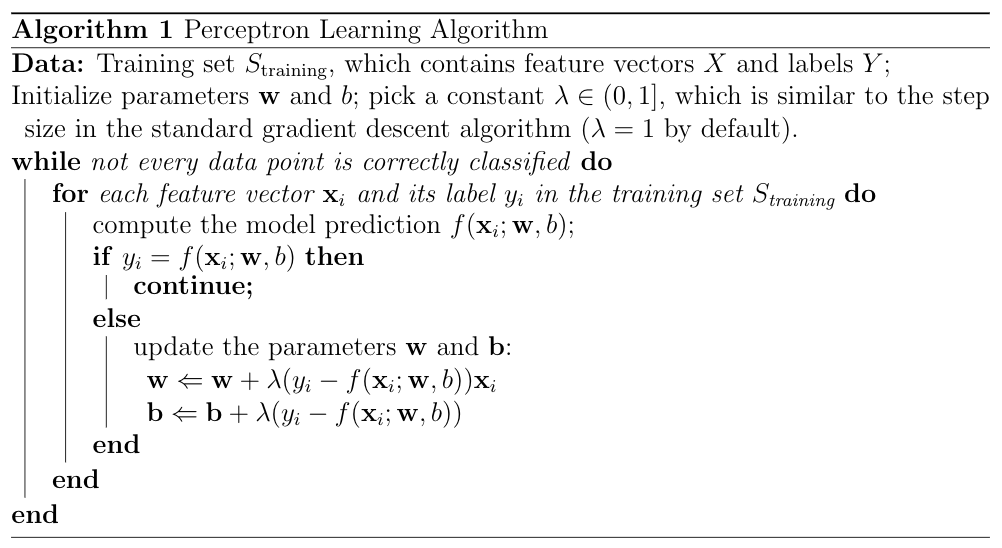
\includegraphics[width=0.9\textwidth]{Images/algorithm_1.png}
        \end{center}

        Please fill out the missing blanks in perceptron.ipynb. Follow the instructions in the skeleton code and report:

        \begin{enumerate}
            \item Your code.
            \item Equation of decision boundary corresponding to the optimal $\w^*$ and $b^*$.
            \item Plot of training set along with decision boundary.
            \item Plot of test set along with decision boundary.
            \item Training error and test error.
            \item Training error curve.
        \end{enumerate}

        \textbf{Hint:}
        \begin{enumerate}
            \item Multiplication inside \texttt{f\_perceptron} is matrix-vector (or vector-vector) multiplication. You can use \texttt{dot}.
            \item Inside the \texttt{update rule}, $\lambda$ and $y_i - f(\x_i; \w, b)$ are scalar while $\x_i$ is a vector. You should consider an element-wise multiplication using \texttt{*}.
        \end{enumerate}

        \begin{verbatim}
def indicator(gt_label, pred_label):
    return int(gt_label != pred_label)
    
def f_perceptron(x, W, b):
    return np.sign(np.dot(x, W) + b)
    
def calc_error(X, Y, W, b):
    errors = np.array([])
    for (xi, yi) in zip(X, Y):
        error = indicator(yi, f_perceptron(xi, W, b))
        errors = np.append(errors, error)
    return np.mean(errors)

# Some settings.
errors = []           # Error history.
lam    = 1            # Lambda which controls the step size.

# Initialization.
W      = np.zeros(2)  # Weight.
b      = 0.0          # Bias.

# Perceptron learning algorithm.
while calc_error(X_train, Y_train, W, b) > 0:
    for xi, yi in zip(X_train, Y_train):   # Iterate over all data points.
        y_pred = f_perceptron(xi, W, b) # Compute the model prediction.
        if yi == y_pred:    # Compare prediction and label.
            continue                       # - If correct, continue.
        else:
            W += lam * (yi - y_pred) * xi
            b += lam * (yi - y_pred)
    errors.append(calc_error(X_train, Y_train, W, b))
        \end{verbatim}

        \newpage

        \begin{soln}
            Decision boundary: $69.600x_0 - 24.200x_1 - 47.000 = 0$.

            \begin{center}
                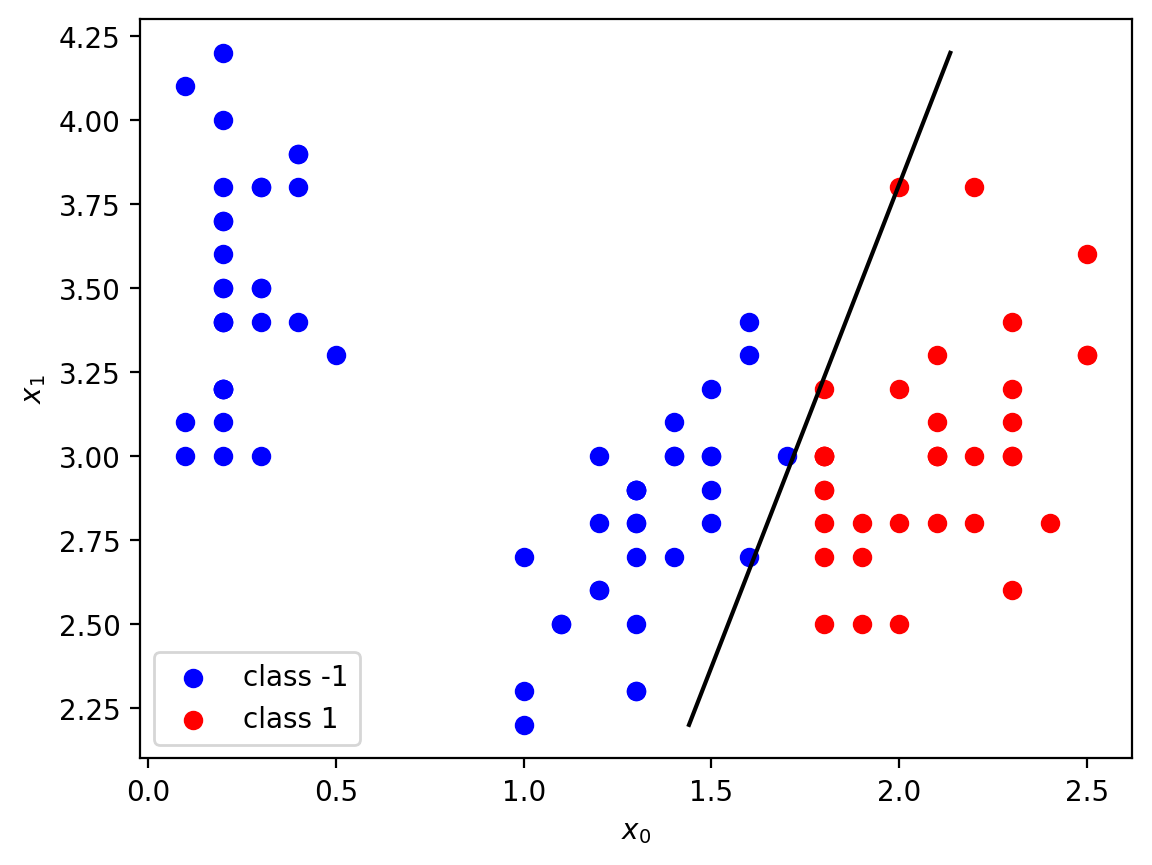
\includegraphics[width=0.5\textwidth]{Images/3.1.1.png}
            \end{center}
            Training error: 0.0

            \begin{center}
                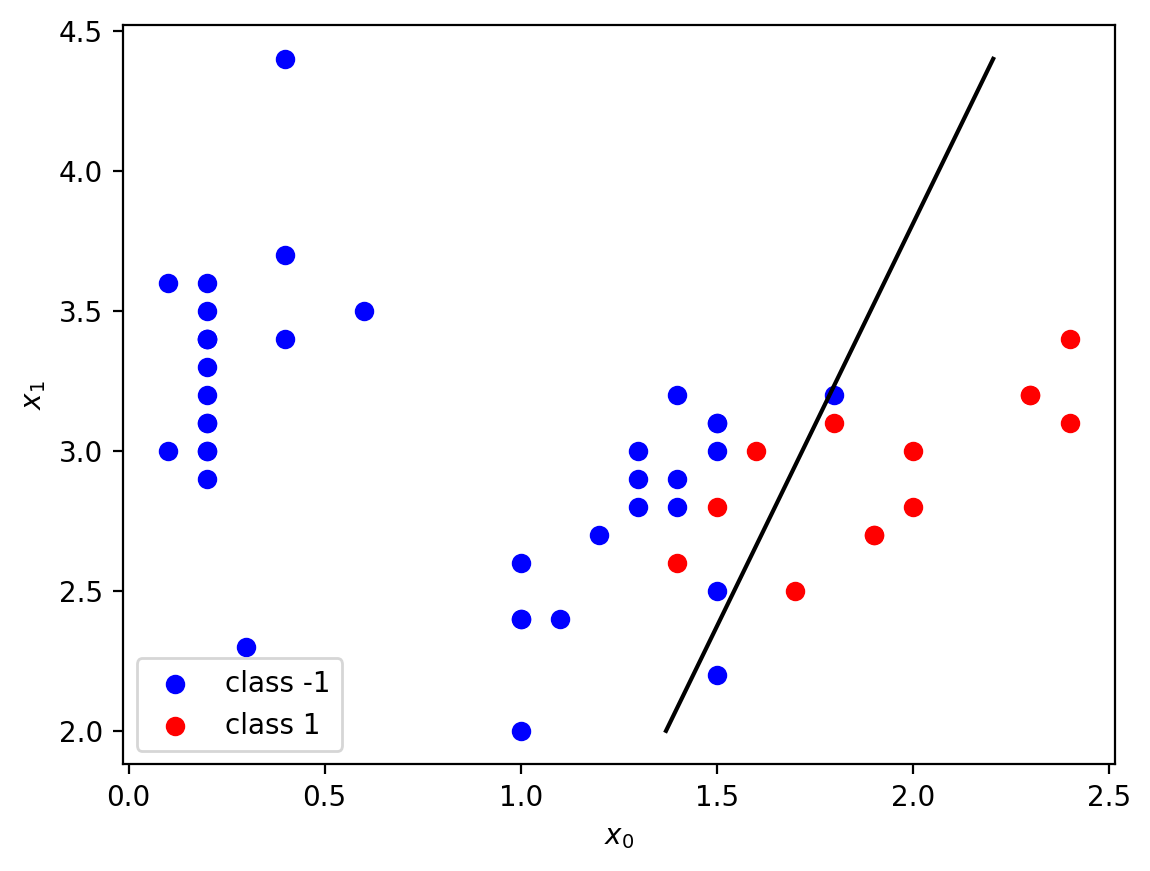
\includegraphics[width=0.5\textwidth]{Images/3.1.2.png}
            \end{center}
            Test error: 0.1

            \begin{center}
                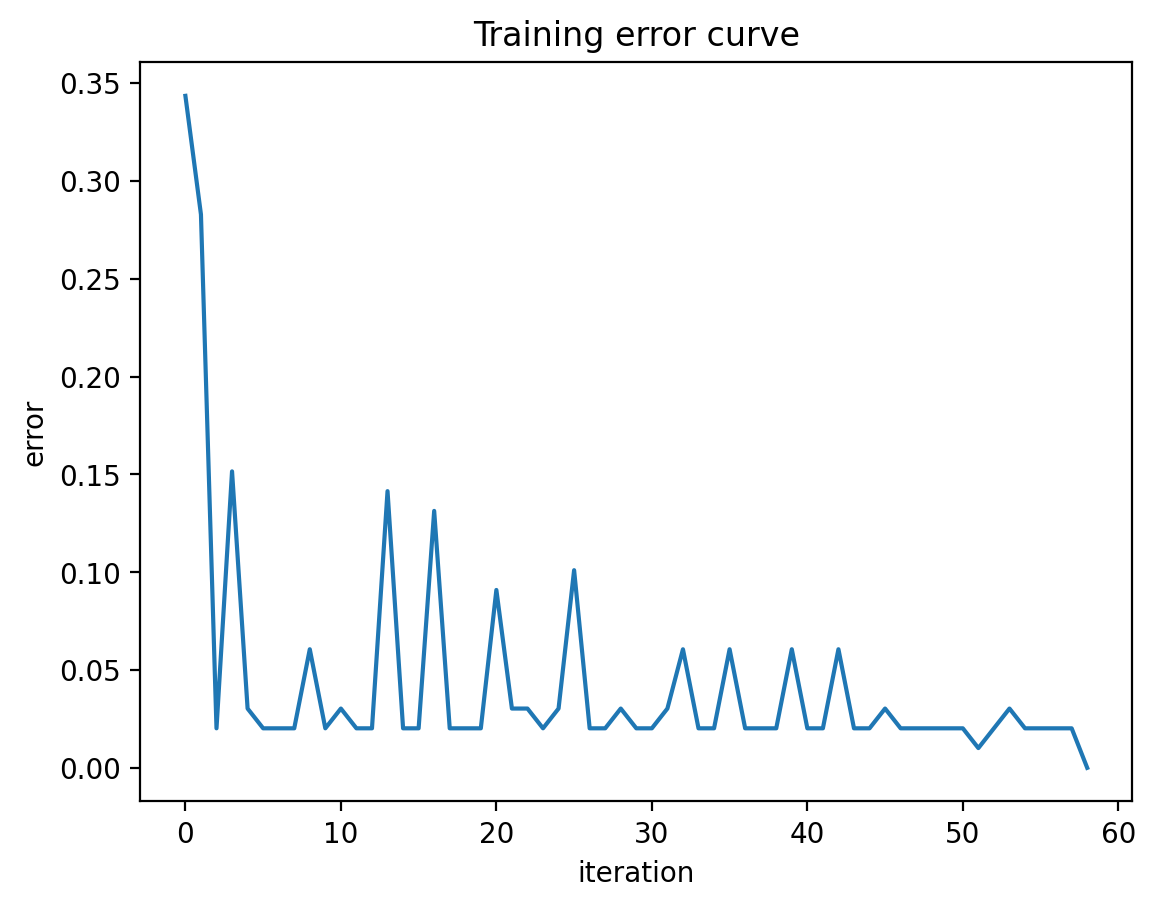
\includegraphics[width=0.5\textwidth]{Images/3.1.3.png}
            \end{center}
        \end{soln}
    \end{subprob}

    \newpage

    \begin{subprob}
        \textbf{(10 points) Perceptron Algorithm - Random Sample}

        In this section, we want to execute the perceptron algorithm in a slightly different way. In the previous section, the perceptron algorithm visits each feature vector $\x_i$ and its label $y_i$ in the training set $S_\text{training}$ in a deterministic order (Line 5 for each feature ...). Now, we want to random sample next $\x_i$ and its label $y_i$ from the training set $S_\text{training}$ with replacement. The new algorithm is shown below:
        
        \begin{center}
            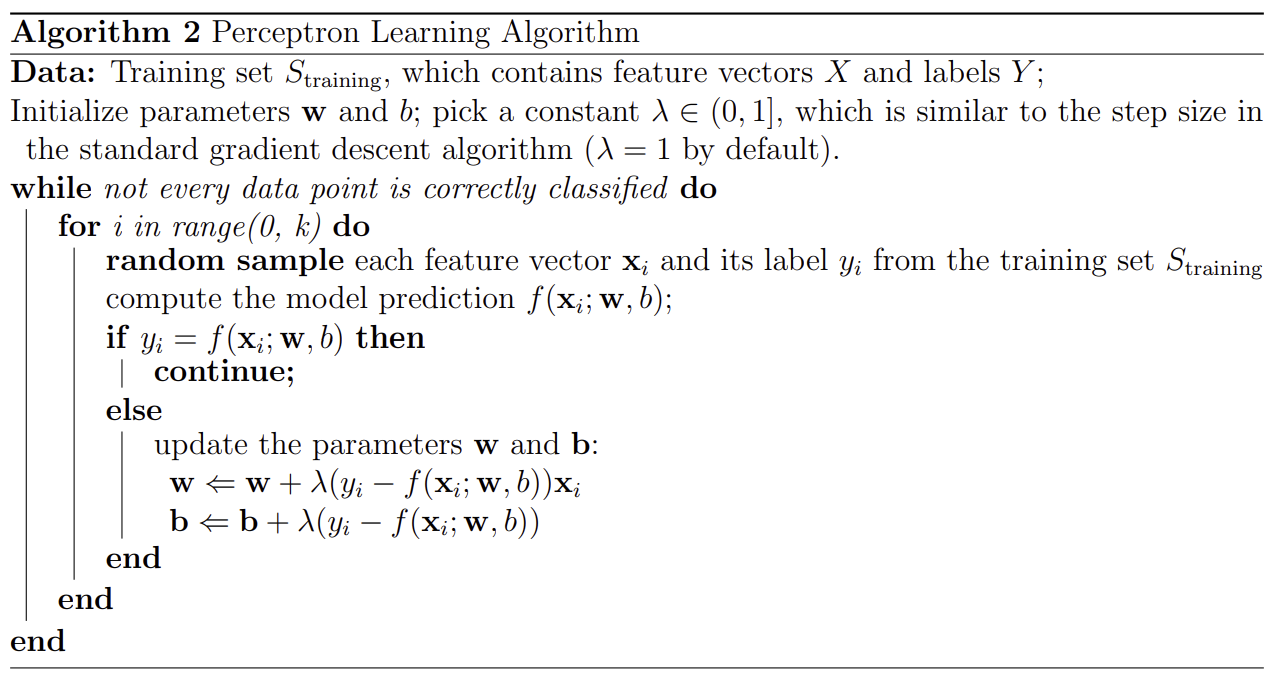
\includegraphics[width=0.9\textwidth]{Images/algorithm_2.png}
        \end{center}

        Please set $k$ = len(training data) and follow the instructions in the skeleton code and report:

        \begin{enumerate}
            \item Your code.
            \item Run your code 3 times and draw 3 training error curves and the curve with deterministic training (Section 3.1). Compare and write your observation between the two sampling methods.
        \end{enumerate}

        \textbf{Hint:} You can randomly sample the indices of training data from 0 to $k - 1$ and then use the index to get the corresponding sample each time. \texttt{random.choices(pop,n)} would return a $n$-sized list of elements chosen from the input list \texttt{pop} with replacement.

        \newpage

        \begin{verbatim}
import random
import matplotlib.pyplot as plt

# Some settings.
errors_random_list = []           # All Error history (3 runs)
lam    = 1            # Lambda which controls the step size.

for _ in range(3):
    # Initialization.
    W      = np.zeros(2)  # Weight.
    b      = 0.0          # Bias.
    k      = len(X_train)
    # Perceptron learning algorithm.
    errors_random = [] # Error history for the current run
    while calc_error(X_train, Y_train, W, b) > 0:
        idxs = np.arange(k)
        np.random.shuffle(idxs)
        for i in range(k):   
            idx = idxs[i]
            xi, yi = X_train[idx], Y_train[idx]
            y_pred = f_perceptron(xi, W, b)
            if yi == y_pred:
                continue
            else:
                W += lam * (yi - y_pred) * xi
                b += lam * (yi - y_pred)
        errors_random.append(calc_error(X_train, Y_train, W, b))
    errors_random_list.append(errors_random)
        \end{verbatim}

        \begin{soln}
            \begin{center}
                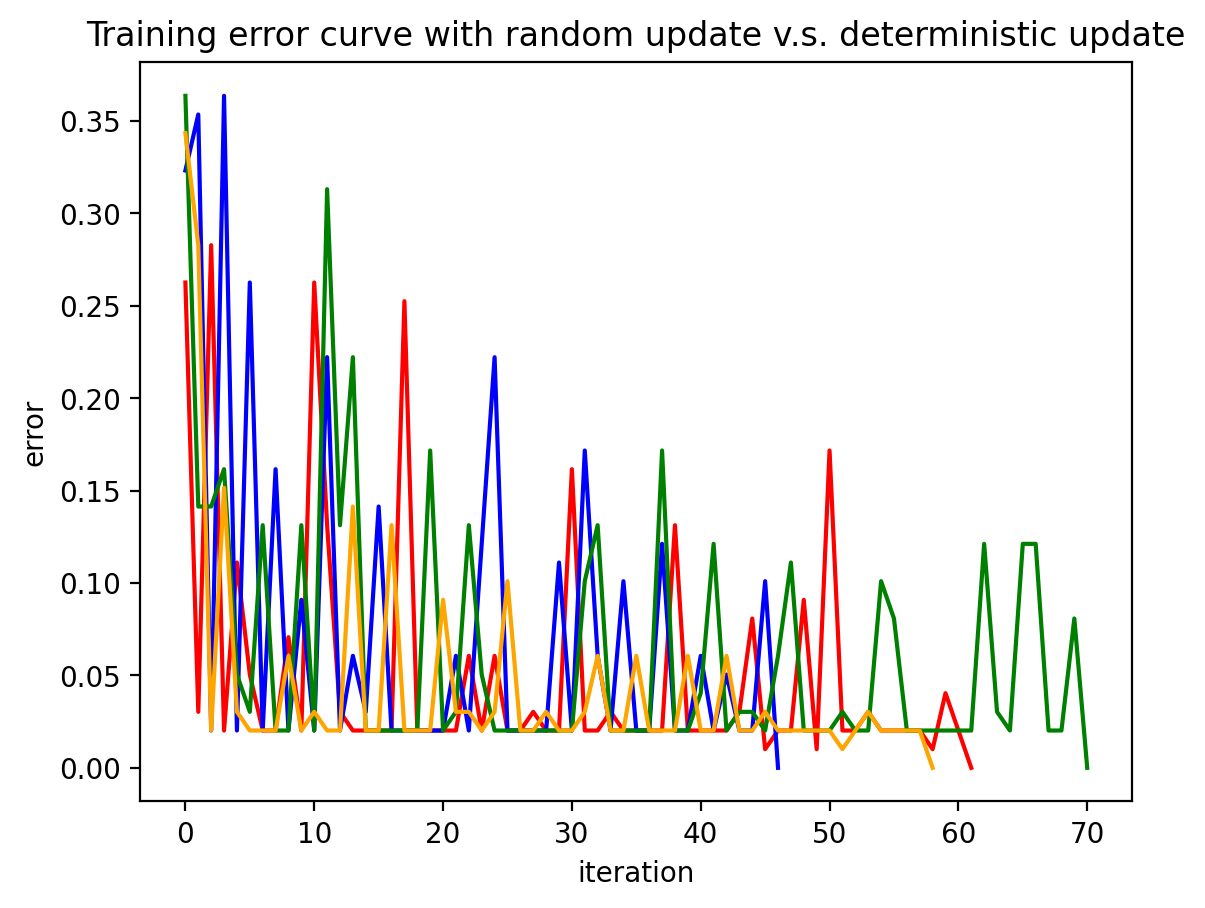
\includegraphics[width=0.5\textwidth]{Images/3.2.png}
            \end{center}
            Clearly, the results of the random sampling method are more volatile than the deterministic method. The deterministic method converged in about 60 iterations, while the random sampling method sometimes took less than 50 iterations and sometimes took more than 70 iterations. This indicates that out of all orders to visit the data points, the deterministic method was quite average.
        \end{soln}
    \end{subprob}
    \end{subprobset}
\end{prob}

\newpage

% --- Problem 4 ---
\begin{prob}[\textbf{(16 points) Circuit Diagram I}]
    The computation of the backpropagation can be nicely visualized with a circuit diagram. Let's consider a complicated expression that involves multiple composite functions, and the function is defined as:
    
    \begin{align}
        f(x, y, z) = (x + y)z
    \end{align}

    We visualize the function with a circuit diagram, which helps us intuitively understand the backpropagation. You can review it from \textit{Fei-Fei Li, Andrej Karpathy}, and \textit{Justin Johnson}'s Stanford CS231n course. Link: http://cs231n.github.io/optimization-2/ The visualization is shown in Fig. 2.

    \begin{figure}[H]
        \centering
        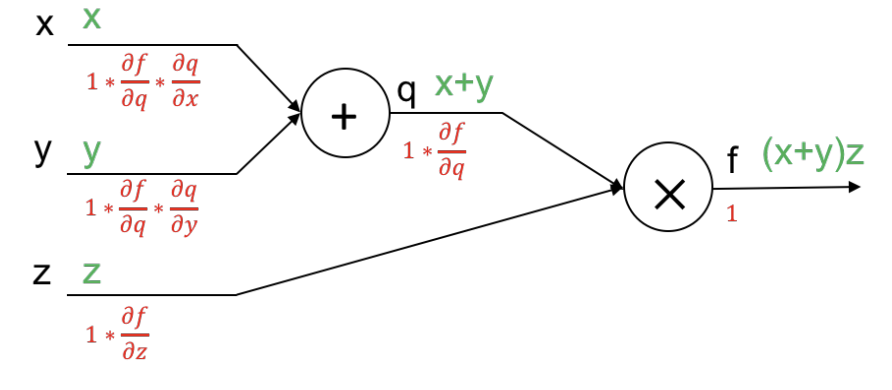
\includegraphics[width=0.7\textwidth]{Images/figure_2.png}
        \caption{Circuit Diagram of the function $f(x, y, z) = (x + y)z$.}
    \end{figure}

    Particularly, this expression can be broken down into two expressions: $q = x + y$ and $f = qz$. According to \textbf{Chain Rule}, the derivative/gradient of $f$ with respect to its inputs $x$, $y$, and $z$ can be calculated easily with the intermediate variable $q$. Although we don't really care about the gradient of $f$ with respect to $q$, but the gradient $\frac{\partial f}{\partial q}$ simplifies the calculation of the gradient.

    Let's take a look at the circuit diagram. The letters in black represent the variables, which are input variables $x$, $y$, $z$, the intermediate variable $q$, and output $f$. The expressions in green represent the current values of the variables respectively, and the expressions in red represent the gradient of $f$ with respect to the particular variables.

    The circuit diagram visualizes how the gradient of $f$ with respect to each variable is calculated. Let's follow the circuit diagram to perform a forward calculation and a backward calculation by hand.

    In Fig. 3, suppose we have three inputs, which are $x = -2$, $y = 5$, and $z = -4$, and the circuit diagram represents the function $f(x, y, z) = (x + y)z$. We follow the steps below to calculate the value and the gradient with respect to each variable in the diagram.

    \begin{enumerate}
        \item $q = x + y = 3$
        \item $f = qz = -12$
        \item $\frac{\partial f}{\partial q} = \frac{\partial (qz)}{\partial q} = z = -4$
        \item $\frac{\partial f}{\partial z} = \frac{\partial (qz)}{\partial z} = q = 3$
        \item $\frac{\partial f}{\partial x} = \frac{\partial f}{\partial q} \cdot \frac{\partial q}{\partial x} = -4 \cdot 1 = -4$
        \item $\frac{\partial f}{\partial y} = \frac{\partial f}{\partial q} \cdot \frac{\partial q}{\partial y} = -4 \cdot 1 = -4$
    \end{enumerate}

    \begin{figure}[H]
        \centering
        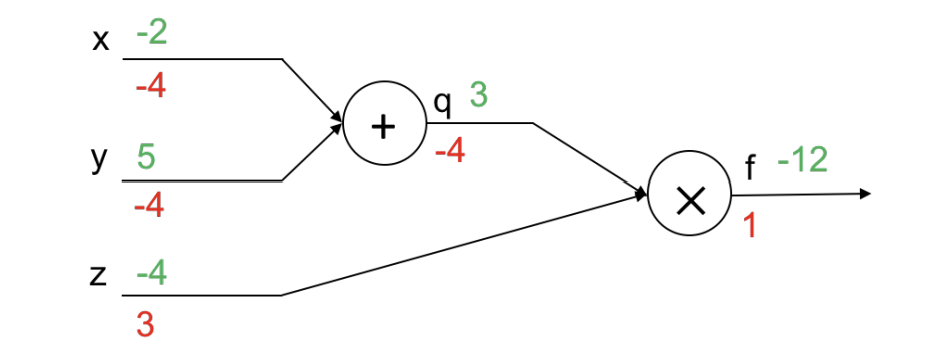
\includegraphics[width=0.7\textwidth]{Images/figure_3.png}
        \caption{The real-valued circuit diagram of the function $f(x, y, z) = (x + y)z$.}
    \end{figure}

    \textbf{Your tasks:}

    The circuit diagram for the function defined below is provided in Fig. 4:
    \begin{align}
        f(x, y, z, w) = \ln[\max(x, y) \times (z + w)],
    \end{align}
    where $\max(x, y)$ takes the maximum value of $x$ and $y$ as output.

    \begin{figure}[H]
        \centering
        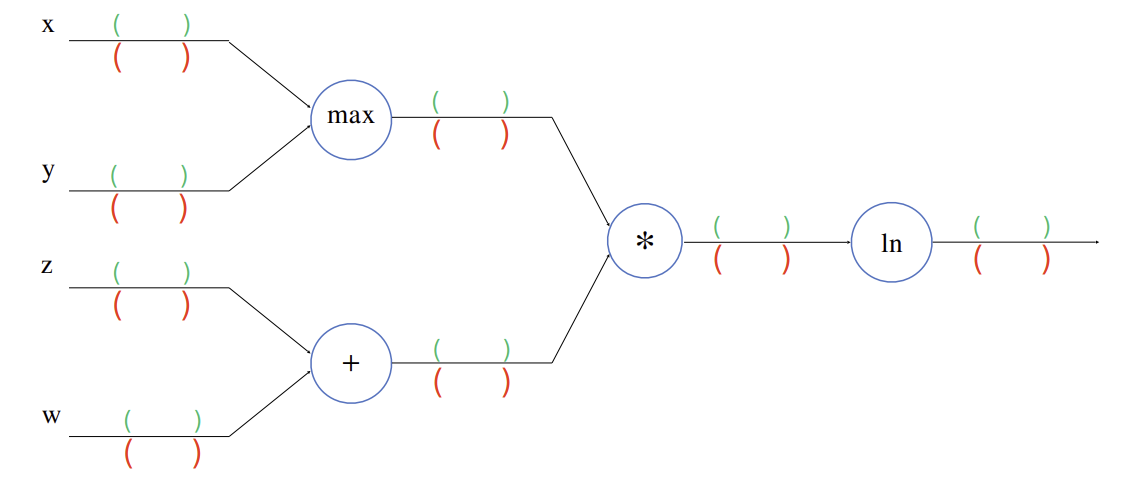
\includegraphics[width=0.7\textwidth]{Images/figure_4.png}
        \caption{Circuit Diagram of the function $f(x, y, z, w)$. We use \texttt{*} to denote the multiplication
        of the two scalar values.}
    \end{figure}

    Suppose the value for each input is $x = 2.5$, $y = 1.5$, $z = 1$ and $w = 3$.

    \newpage
    
    \begin{subprobset}
    \begin{subprob}
        \textbf{(8 points)} Perform the forward computation of the function $f$, and fill-in the circuit diagram in Fig. 4 with your calculated values.

        \begin{soln}
            \begin{center}
                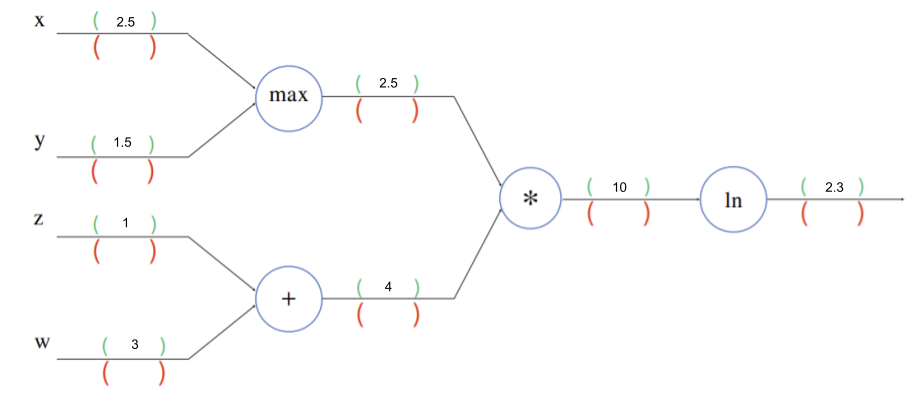
\includegraphics[width=0.7\textwidth]{Images/4.1.png}
            \end{center}
            $q = \max(x, y) = 2.5$, $p = z + w = 4$, $r = qp = 10$, $f = \ln(r) = \ln(10) \approx 2.3$
        \end{soln}
    \end{subprob}

    \begin{subprob}
        \textbf{(8 points)} Perform the backward computation of the function $f$, and fill-in the circuit diagram in Fig. 4 with your calculated gradients.

        \begin{soln}
            \begin{center}
                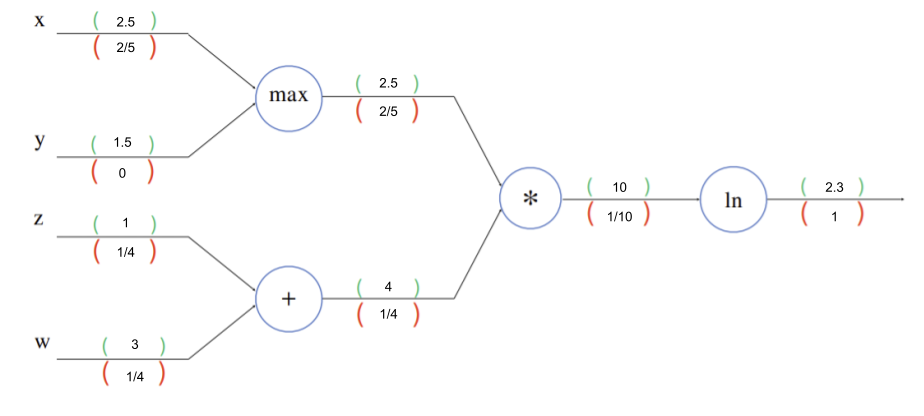
\includegraphics[width=0.7\textwidth]{Images/4.2.png}
            \end{center}
            \begin{align*}
                \frac{\partial f}{\partial r} &= \frac{\partial \ln(r)}{\partial r} = \frac{1}{r} = \frac{1}{10}, \\
                \frac{\partial f}{\partial q} &= \frac{\partial f}{\partial r} \cdot \frac{\partial r}{\partial q} = \frac{1}{10} \cdot p = \frac{2}{5}, \\
                \frac{\partial f}{\partial p} &= \frac{\partial f}{\partial r} \cdot \frac{\partial r}{\partial p} = \frac{1}{10} \cdot q = \frac{1}{4}, \\
                \frac{\partial f}{\partial x} &= \frac{\partial f}{\partial q} \cdot \frac{\partial q}{\partial x} = \frac{2}{5} \cdot \underbrace{int(x > y)}_{1} = \frac{2}{5}, \\
                \frac{\partial f}{\partial y} &= \frac{\partial f}{\partial q} \cdot \frac{\partial q}{\partial y} = \frac{2}{5} \cdot \underbrace{int(y > x)}_{0} = 0, \\
                \frac{\partial f}{\partial z} &= \frac{\partial f}{\partial p} \cdot \frac{\partial p}{\partial z} = \frac{1}{4} \cdot 1 = \frac{1}{4}, \\
                \frac{\partial f}{\partial w} &= \frac{\partial f}{\partial p} \cdot \frac{\partial p}{\partial w} = \frac{1}{4} \cdot 1 = \frac{1}{4}
            \end{align*}
        \end{soln}
    \end{subprob}
    \end{subprobset}
\end{prob}

% --- Problem 5 ---
\begin{prob}[\textbf{(16 points) Logistic Regression}]
    Assume in a binary classification problem, we need to predict a binary label $y \in \{-1, +1\}$ for a feature vector $\x = [x_0, x_1]^\top$. In logistic regression, we can reformulate the binary classification problem in a probabilistic framework: We aim to model the distribution of classes given the input feature vector $\x$. Specifically, we can express the conditional probability $p(y|\x)$ parameterized by $(\w, b)$ using a logistic function. Assume the probability of the positive prediction $p(y = +1|\x)$ is represented as:

    \begin{align}
        p(y = +1|\x) = \frac{1}{1 + e^{-(\w^\top \x + b)}}
    \end{align}

    \begin{subprobset}
    \begin{subprob}
        \textbf{(8 points) Basic Formulation} 
        
        \begin{enumerate}
            \item Please derive the formulation of $p(y = -1|\x)$.
            \item Please show that $p(y|\x) = \frac{1}{1 + e^{-y(\w^\top \x + b)}}$.
        \end{enumerate}

        \begin{soln}
            Using the property of the sigmoid function, we have:
            \begin{enumerate}
                \item $p(y = -1|\x) = 1 - p(y = +1|\x) = 1 - \sigma(\w^\top \x + b) = \sigma(-\w^\top \x - b) = \frac{1}{1 + e^{\w^\top \x + b}}$
                \item $p(y|\x) = \sigma(y(\w^\top \x + b)) = \frac{1}{1 + e^{-y(\w^\top \x + b)}}$
            \end{enumerate}
            We can see that if $y = +1$, then $p(y = +1|\x) = \sigma(\w^\top \x + b)$. If $y = -1$, then $p(y = -1|\x) = \sigma(-\w^\top \x - b)$ which matches our derivation.
        \end{soln}
    \end{subprob}

    \newpage

    \begin{subprob}
        \textbf{(8 points) Derive Gradient}

        Given a training dataset $S_\text{training} = \{(\x_i, y_i), i = 1, \ldots, n\}$, we wish to optimize the negative log-likelihood loss $L(\w, b)$ of the logistic regression model defined above:

        \begin{align}
            L(\w, b) = -\sum_{i=1}^n \ln p(y_i|\x_i)
        \end{align}

        where $p_i = p(y_i|\x_i)$. The optimal weight vector $\w$ and bias $b$ are used to build the
        logistic regression model:

        \begin{align}
            \w^*, b^* = \arg \min_{w, b} L(w, b)
        \end{align}

        In this problem, we attempt to obtain the optimal parameters $\w^*$ and $b^*$ by using a standard gradient descent algorithm.

        \begin{enumerate}[label=(\alph*)]
            \item Please show that $\frac{\partial L(\w, b)}{\partial \w} = -\sum_{i=1}^n (1 - p_i) y_i \x_i$.
            \item Please show that $\frac{\partial L(\w, b)}{\partial b} = -\sum_{i=1}^n (1 - p_i) y_i$.
        \end{enumerate}

        \begin{soln}
            Here we use the fact that the derivative of the sigmoid function is $\sigma'(z) = \sigma(z)(1 - \sigma(z))$, so let $z_i = y_i(\w^\top \x_i + b)$ hence 
            
            \[
                \frac{\partial p_i}{\partial z_i} = \sigma(z_i)(1 - \sigma(z_i)) = p_i(1 - p_i)
            \] 
            
            Now, using the chain rule, we have 
            \[
                \frac{\partial \ln p_i}{\partial z_i} = \frac{\partial \ln p_i}{\partial p_i} \cdot \frac{\partial p_i}{\partial z_i} = \frac{1}{p_i}p_i(1 - p_i) = 1 - p_i
            \] 
            
            Finally, we use chain rule again to find 
            
            \[
                \frac{\partial L}{\partial \w} = -\sum_{i=1}^n \frac{\partial \ln p_i}{\partial z_i} \cdot \frac{\partial z_i}{\partial \w} = -\sum_{i=1}^n (1 - p_i) y_i \x_i
            \]
            \[
                \frac{\partial L}{\partial b} = -\sum_{i=1}^n \frac{\partial \ln p_i}{\partial z_i} \cdot \frac{\partial z_i}{\partial b} = -\sum_{i=1}^n (1 - p_i) y_i
            \]
        \end{soln}
    \end{subprob}
    \end{subprobset}
\end{prob}

\newpage

% --- Problem 6 ---
\begin{prob}[\textbf{(10 points) Multi-Layer Neural Networks}]
    \begin{figure}[H]
        \centering
        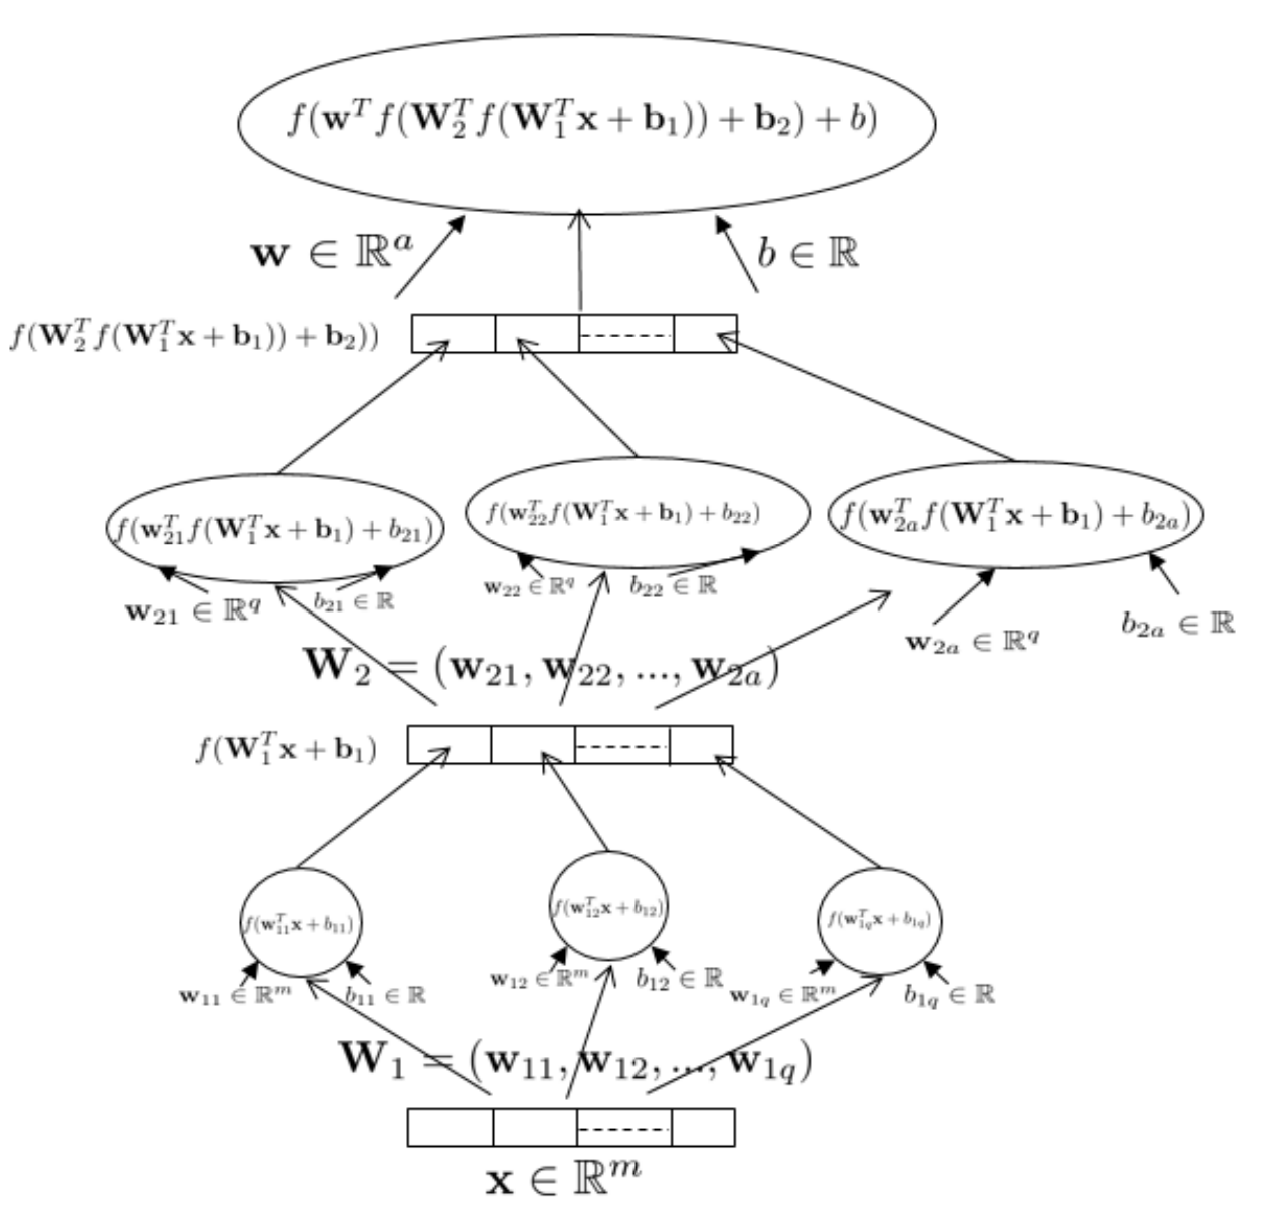
\includegraphics[width=0.9\textwidth]{Images/figure_5.png}
        \caption{A multi-layer feedforward neural networks structure.}
    \end{figure}

    \newcommand{\W}{\mathbf{W}}
    
    Figure 5 shows a multi-layer feedforward neural network structure, where $m = 5$, $q = 8$, and $a = 6$. Note that function $f(\W)$ performs element-wise operations on an input matrix $\W$.

    \newpage

    Please provide the sizes of the variables listed below.
    \begin{enumerate}
        \item $x$:
        \item $\W_1$:
        \item $b_1$:
        \item $f(W_1^\top x + b_1)$:
        \item $\W_2$:
        \item $b_2$:
        \item $f(\W_2^\top f(\W_1^\top x + b_1) + b_2)$:
        \item $w$:
        \item $b$:
        \item $f(w^\top f(\W_2^\top f(\W_1^\top x + b_1) + b_2) + b)$:
    \end{enumerate}

    \begin{soln}
        \begin{enumerate}
            \item $x \in \R^5$
            \item $\W_1 \in \R^{5 \times 8}$
            \item $b_1 \in \R^8$
            \item $f(\W_1^\top x + b_1): \R^8 \to \R^8$
            \item $\W_2 \in \R^{8 \times 6}$
            \item $b_2 \in \R^6$
            \item $f(\W_2^\top f(\W_1^\top x + b_1) + b_2): \R^6 \to \R^6$
            \item $w \in \R^6$
            \item $b \in \R$
            \item $f(w^\top f(\W_2^\top f(\W_1^\top x + b_1) + b_2) + b): \R \to \R$
        \end{enumerate}
    \end{soln}
\end{prob}

\newpage

% --- Problem 7 ---
\begin{prob}[\textbf{(10 points) Number of Parameters}]
    Consider a one-hidden-layer network with 3-dimensional input, 2-dimensional output, and 5 hidden units as shown in Figure 6.

    \begin{subprobset}
    \begin{subprob}
        \textbf{(2 points)} How many neurons (nodes) are there in a neural network? Do not count the input layer.

        \begin{figure}[H]
            \centering
            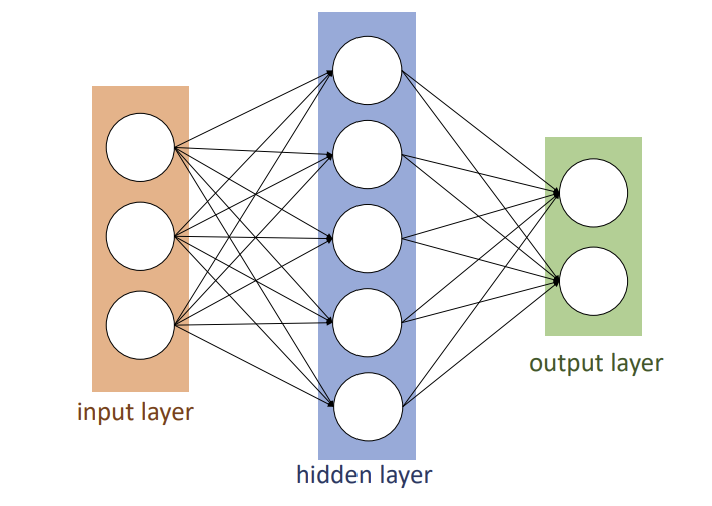
\includegraphics[width=0.7\textwidth]{Images/figure_6.png}
            \caption{Question 7.}
        \end{figure}

        \begin{soln}
            There are 5 in the hidden layer and 2 in the output layer which is 7 neurons in total.
        \end{soln}
    \end{subprob}

    \begin{subprob}
        \textbf{(2 points)} How many weights (edges) are there in the network?

        \begin{soln}
            There are $3 \times 5$ weights to the first layer and $5 \times 2$ weights to the second layer which is 25 weights in total.
        \end{soln}
    \end{subprob}

    \begin{subprob}
        \textbf{(3 points)} How many learnable parameters are there in total in the network? Include the bias parameters in your answer.

        \begin{soln}
            There are 25 weights and 7 neurons with biases which is 32 parameters in total.
        \end{soln}
    \end{subprob}

    \begin{subprob}
        \textbf{(3 points)} Now let's generalize the result from part 3. How many parameters are there in a one-hidden-layer network with $D_x$-dimensional input, $D_y$-dimensional output, and $H$ hidden units? Include the bias parameters in your answer.

        \begin{soln}
            There are $D_x \times H$ weights to the first layer and $H \times D_y$ weights to the second layer which is $D_x \times H + H \times D_y + H + D_y$ parameters in total.
        \end{soln}
    \end{subprob}
    \end{subprobset}
\end{prob}
\end{probset}
\end{document}